\subsection{Capturas Reais da Plataforma em Operação Retrospectiva}
\label{subsec:capturas-reais-plataforma}

Para evidenciar a integração efetiva entre a camada de engenharia de dados, os detectores multivisão e as interfaces de investigação sem depender de protótipos ilustrativos, a TUI em terminal e o Cockpit Analítico Web foram executados localmente sobre a suíte retrospectiva validada em \texttt{latest\_suite.json} (corte OOT \texttt{19/11/2026}, \texttt{run\_id = 20261123\_124416\_146\_oot\_multiview}, 65.686 UCs anonimizadas). Todas as saídas mantêm tema claro acadêmico e mascaramento LGPD de identificadores, circuitos e concessionária. Ressalta-se que estas capturas demonstram o \emph{funcionamento do software sobre dados históricos reais}, sem implicar validação presencial por ordens de serviço em campo.

\begin{figure}[htbp]
  \centering
  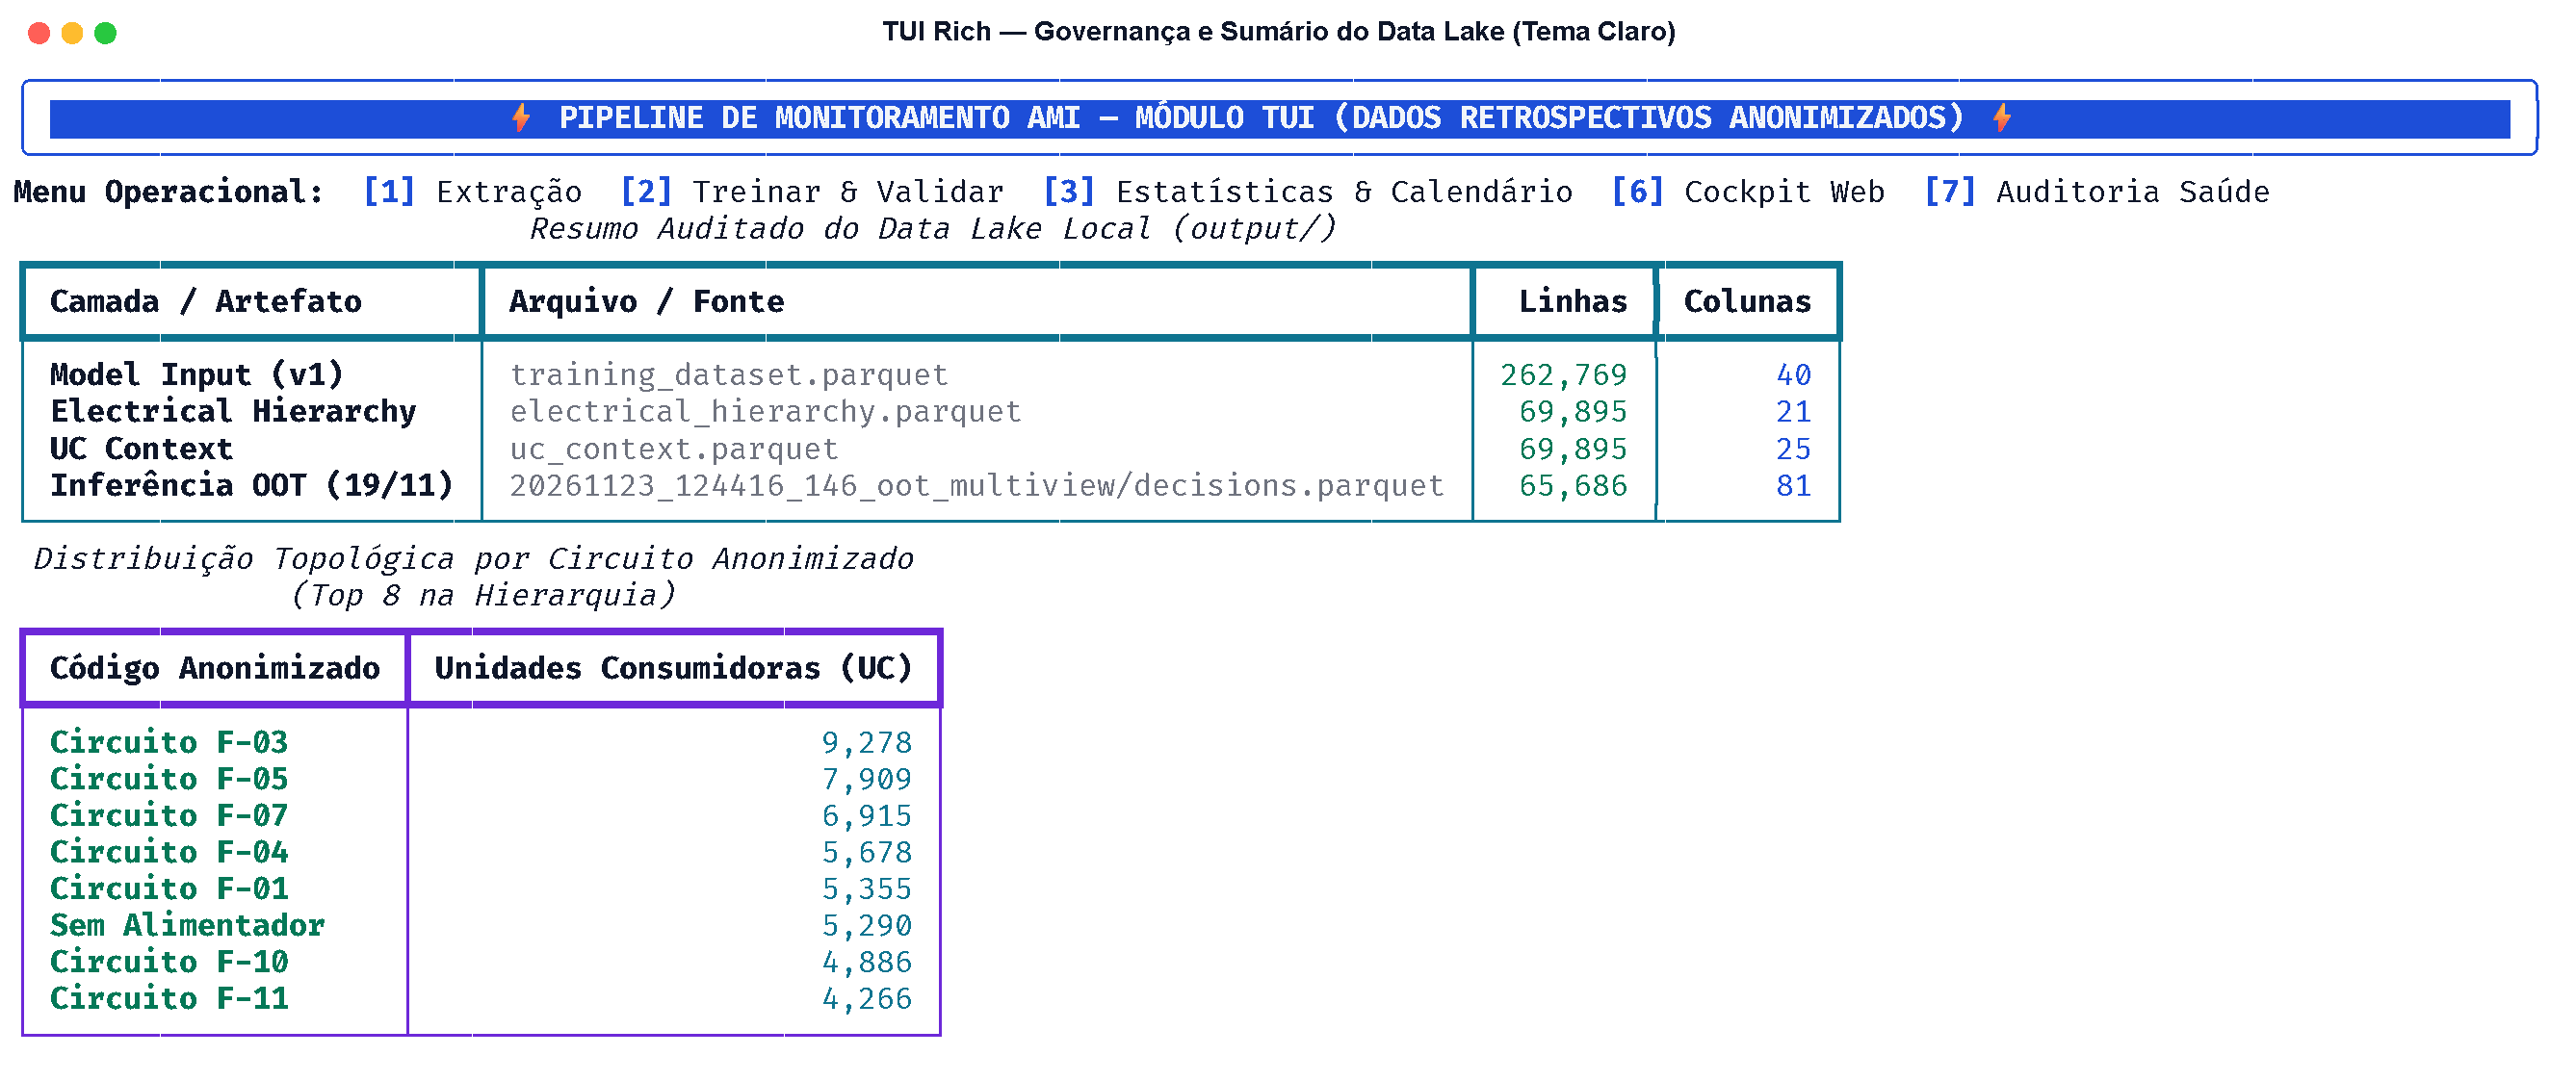
\includegraphics[width=0.96\textwidth]{manuscript_figures/platform_interfaces/fig_4_4a_tui_menu_governanca.pdf}
  \caption{Interface de terminal (TUI Rich exportada em SVG vetorial) executada sobre os artefatos reais do Data Lake e da suíte validada, exibindo cardinalidade das camadas e distribuição topológica anonimizada por circuito.}
  \label{fig:tui-menu-governanca}
\end{figure}

\begin{figure}[htbp]
  \centering
  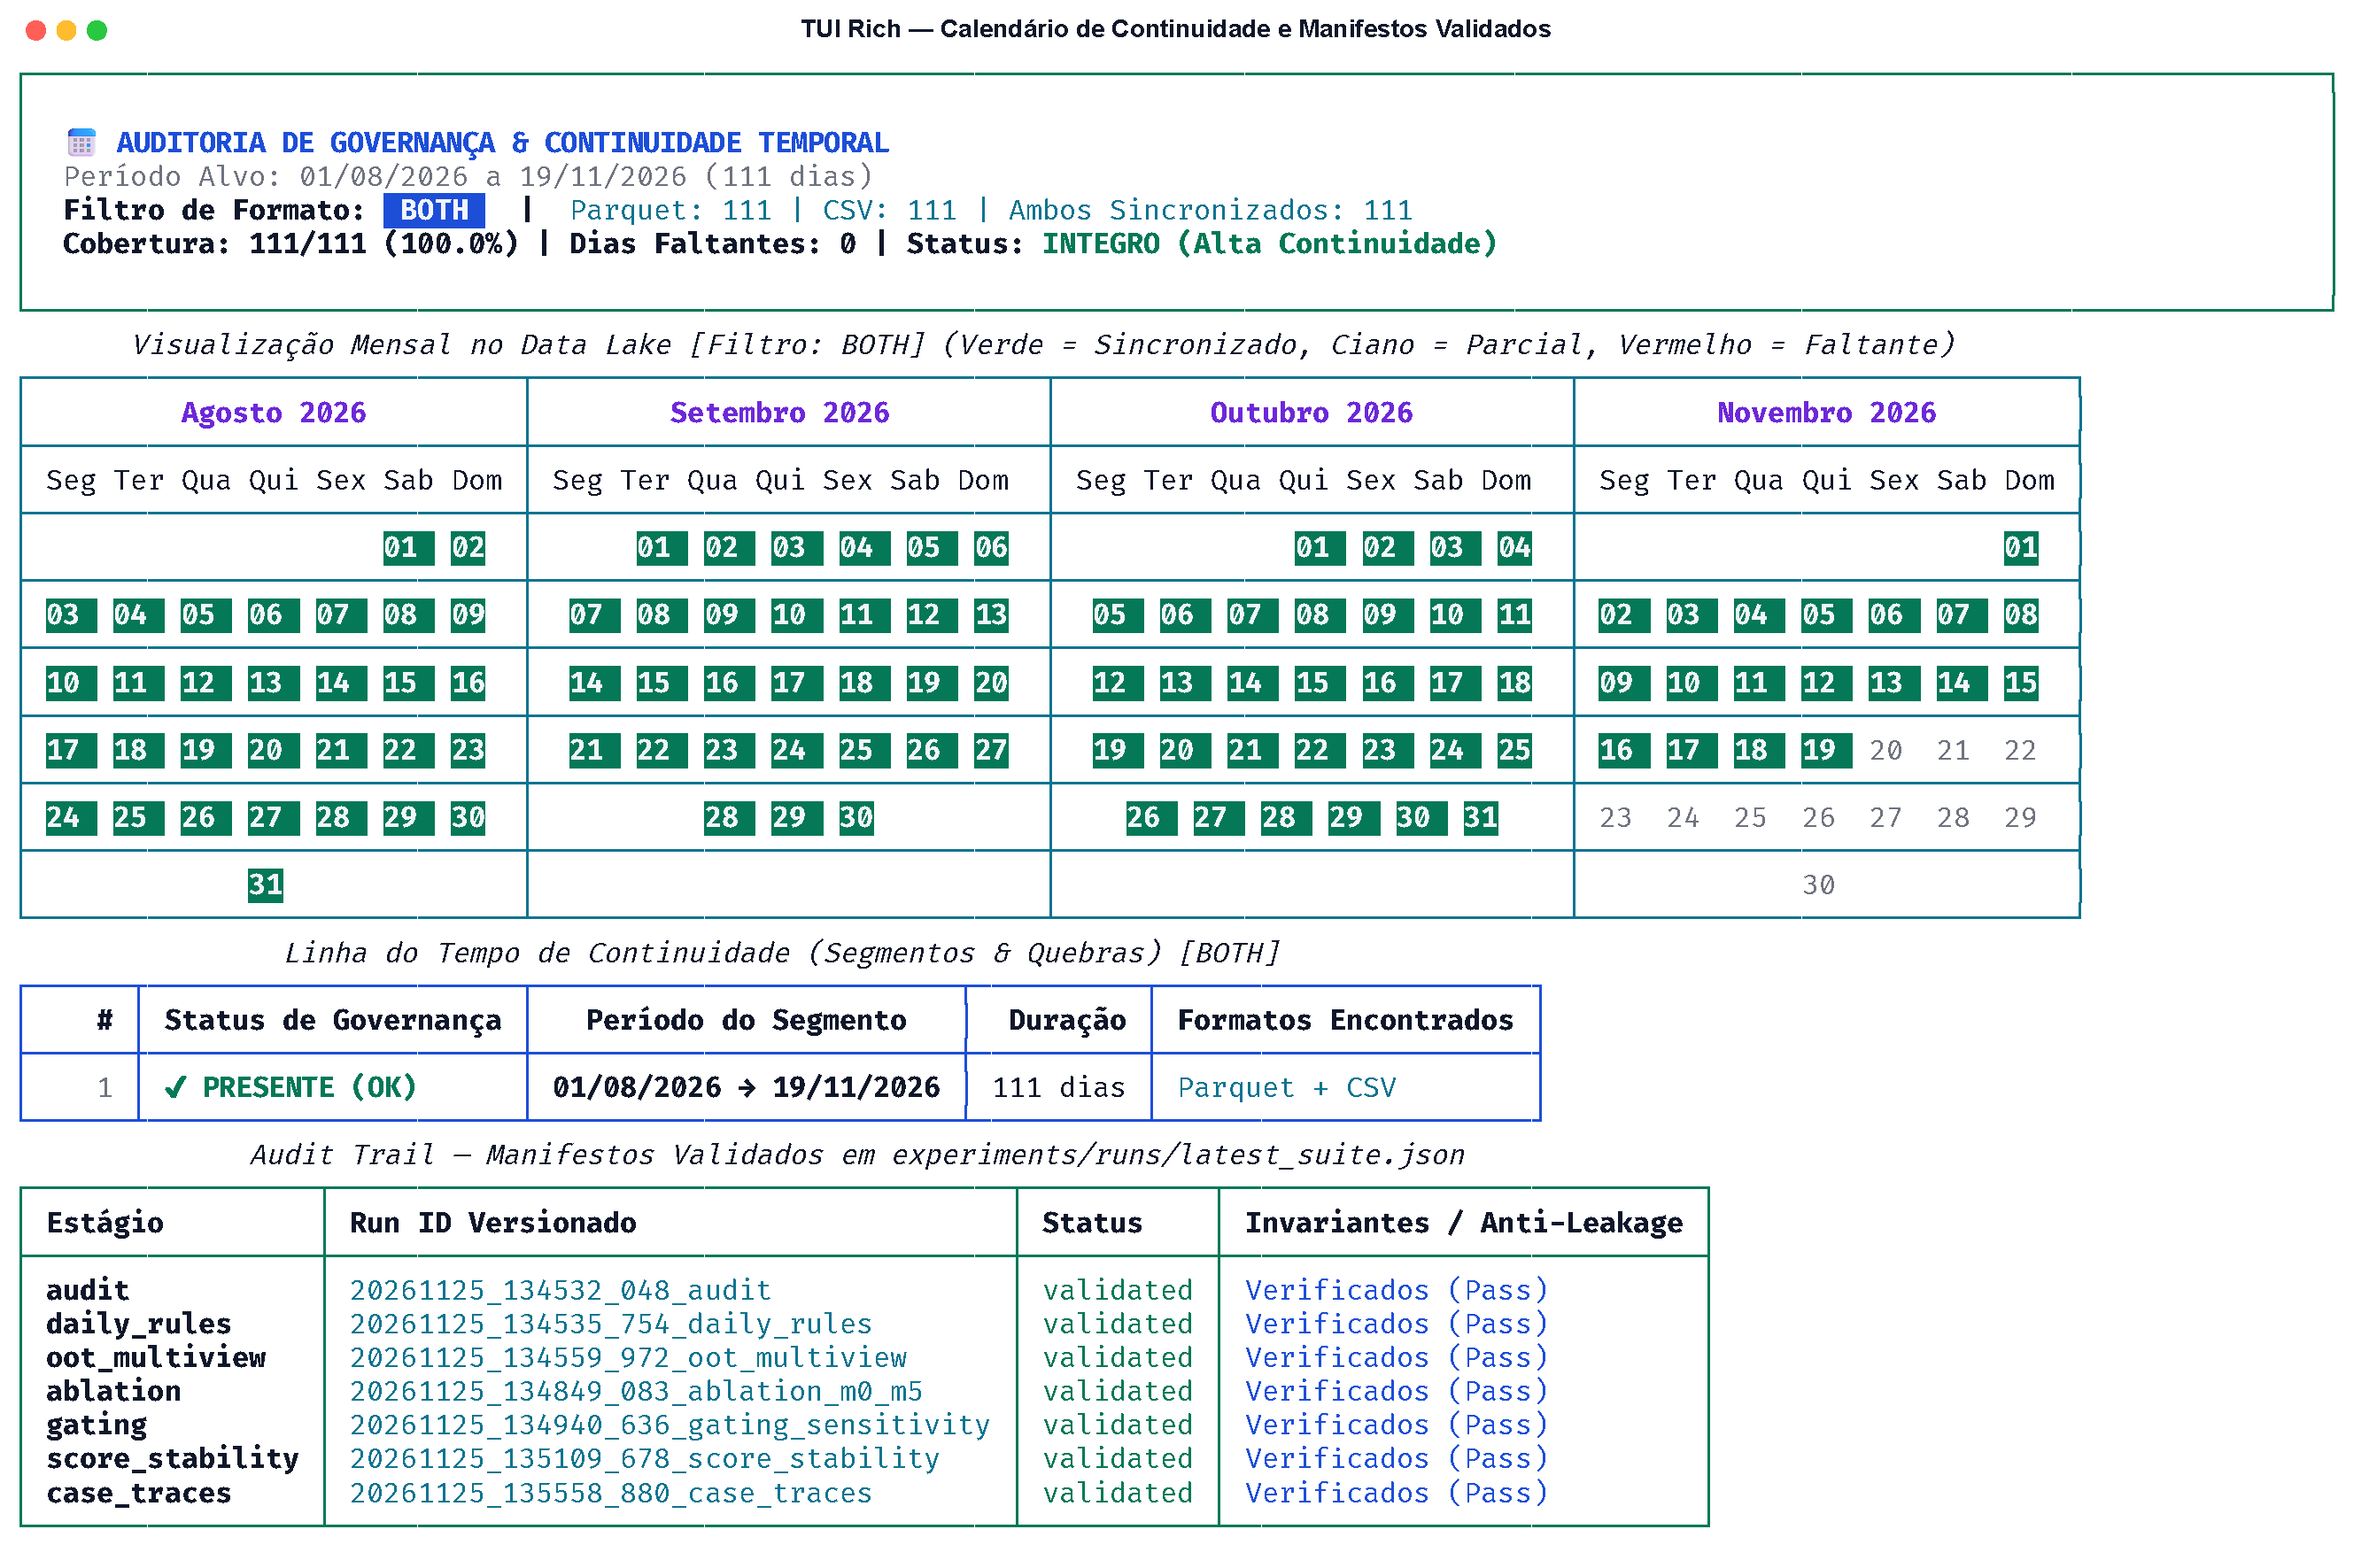
\includegraphics[width=0.96\textwidth]{manuscript_figures/platform_interfaces/fig_4_4b_tui_calendario_auditoria.pdf}
  \caption{Calendário real de continuidade temporal (111 dias íntegros entre 01/08/2026 e 19/11/2026) renderizado por \texttt{render\_continuity\_calendar} e trilha de auditoria dos manifestos ativos.}
  \label{fig:tui-calendario-auditoria}
\end{figure}

As Figuras~\ref{fig:tui-menu-governanca} e~\ref{fig:tui-calendario-auditoria} comprovam que a arquitetura de dados assegura rastreabilidade estrutural antes de qualquer inferência estatística. O calendário verifica continuidade integral de partições em formato dual (\texttt{Parquet} e \texttt{CSV}), enquanto a tabela de manifestos registra invariantes sem vazamento temporal.

\begin{figure}[htbp]
  \centering
  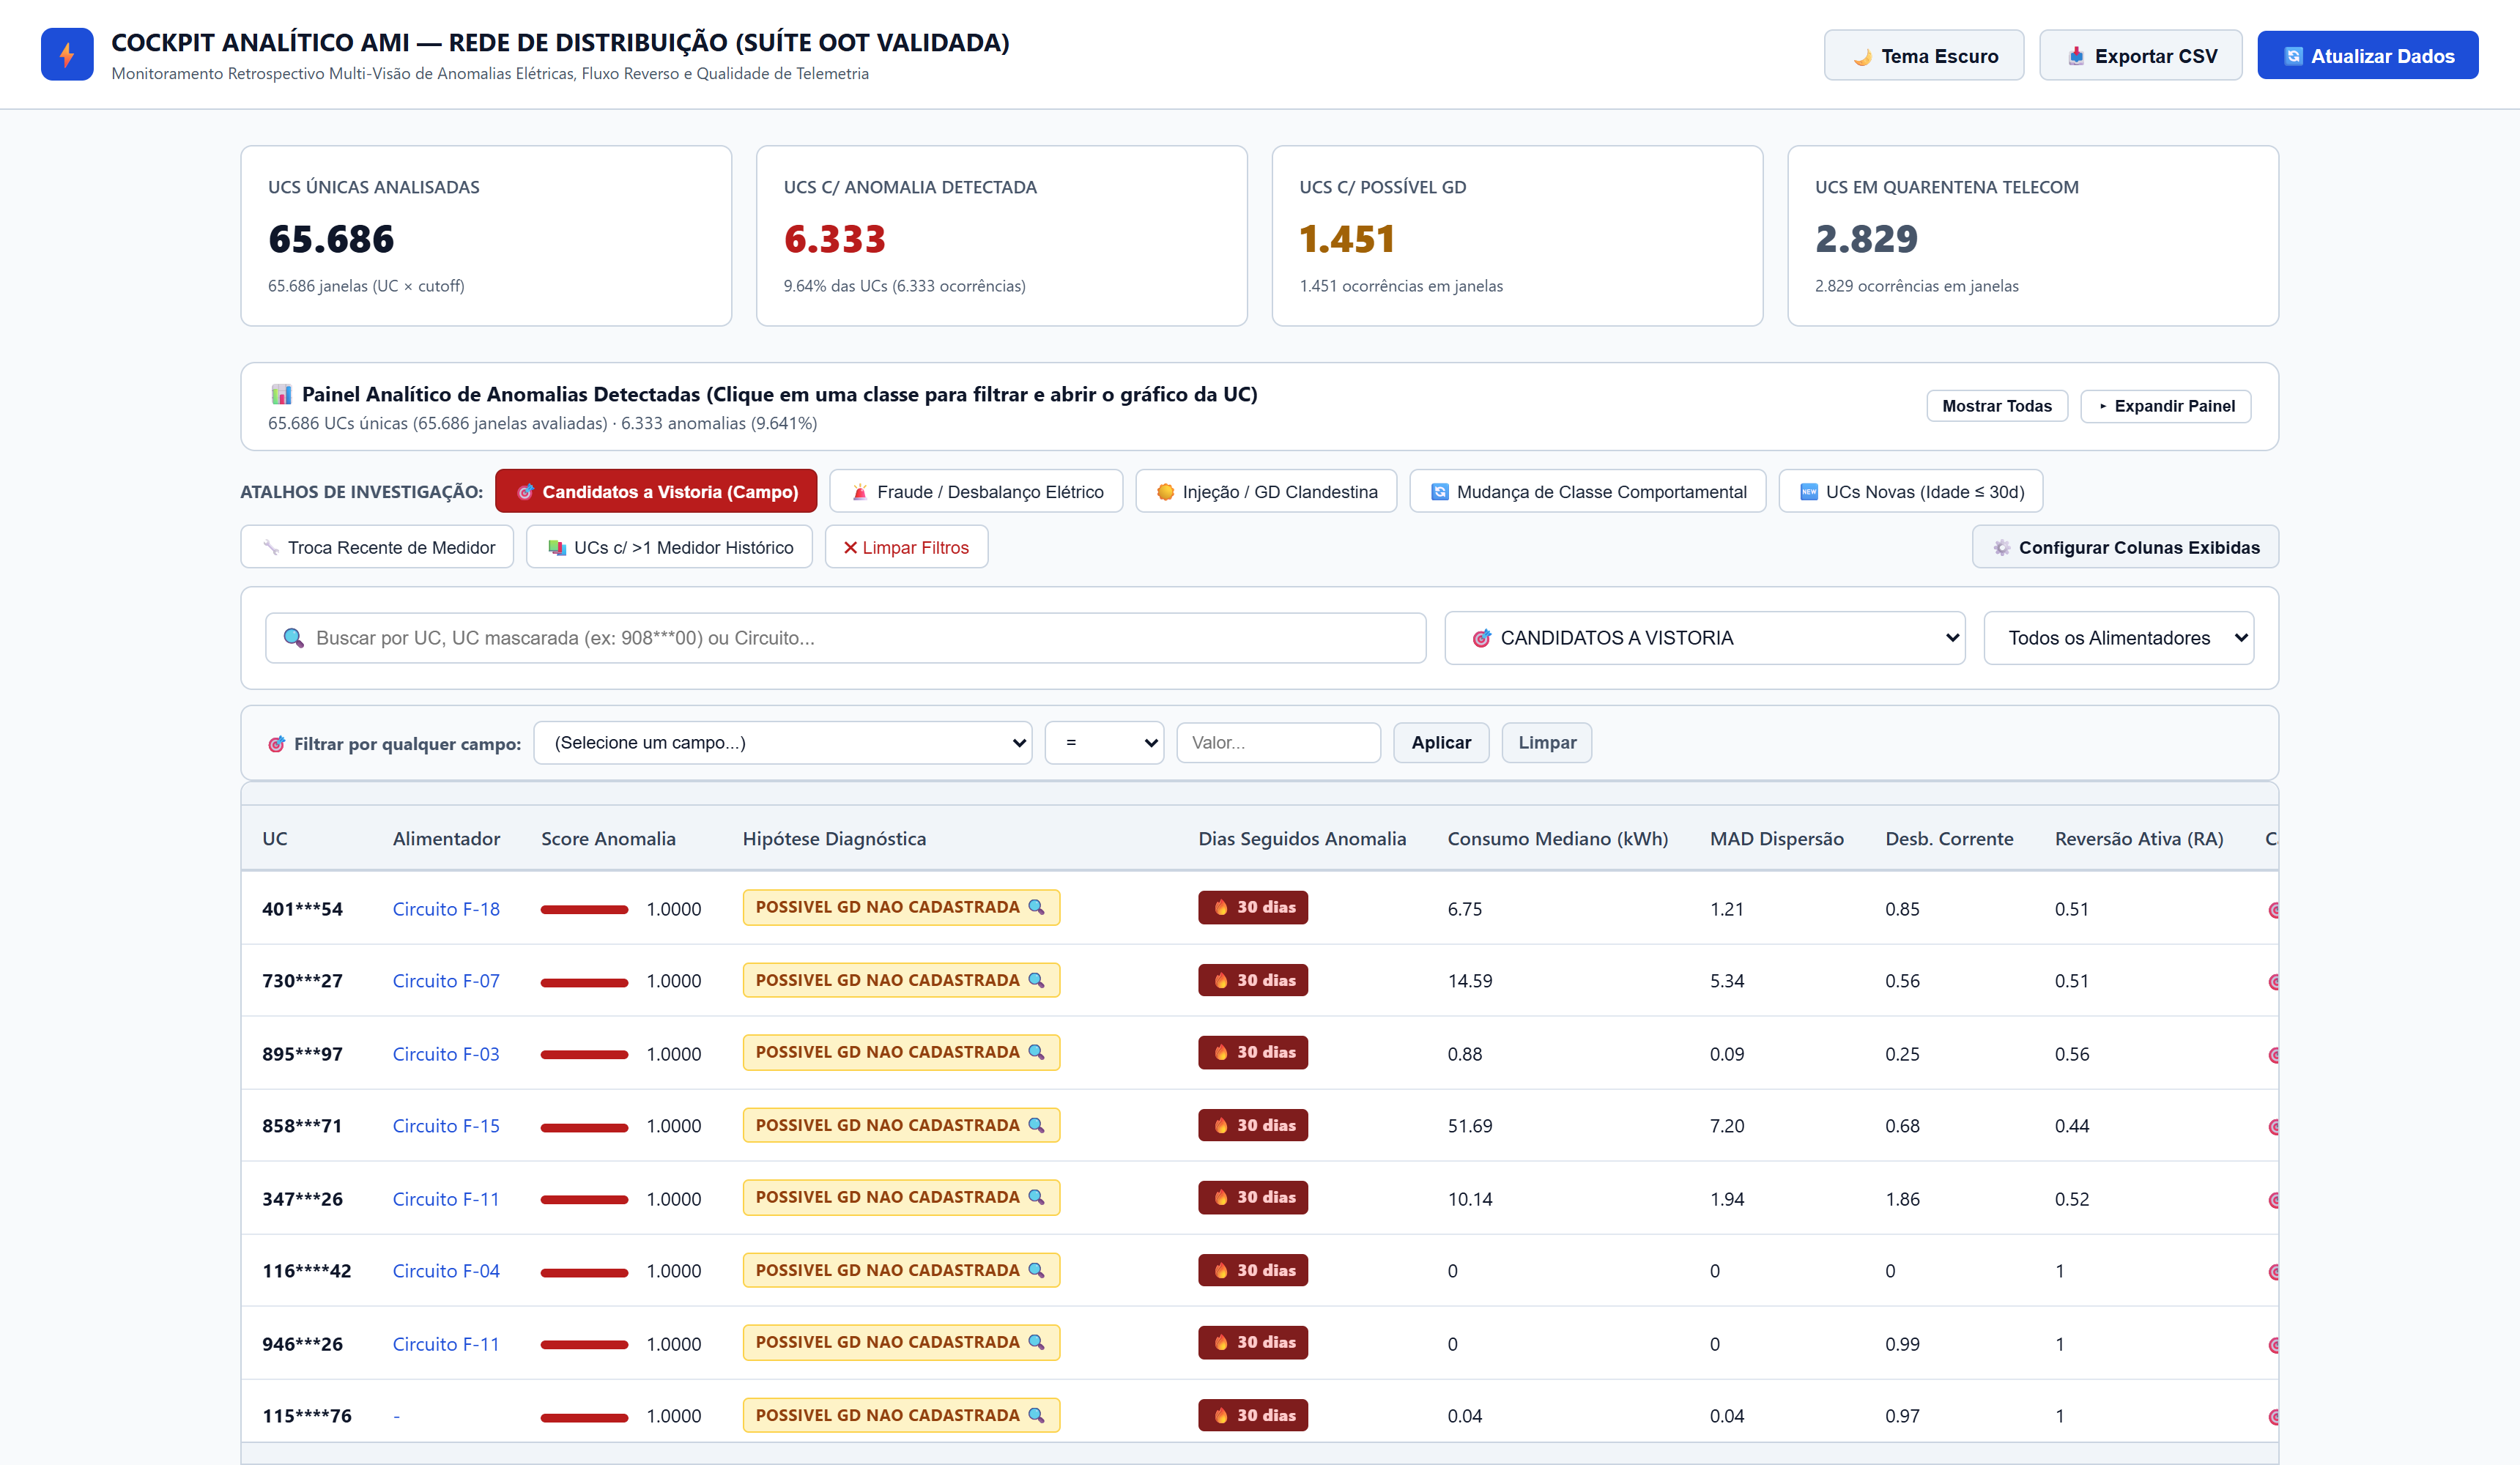
\includegraphics[width=0.98\textwidth]{manuscript_figures/platform_interfaces/fig_4_4c_cockpit_carteira_candidatos.png}
  \caption{Cockpit Analítico Web capturado via Playwright sobre o corte OOT validado (\texttt{65.686} UCs totais; \texttt{6.333} candidatas à vistoria; \texttt{1.451} possíveis GD; \texttt{2.829} em quarentena de telecomunicação) com filtro de carteira priorizada ativo.}
  \label{fig:cockpit-carteira-candidatos}
\end{figure}

\begin{figure}[htbp]
  \centering
  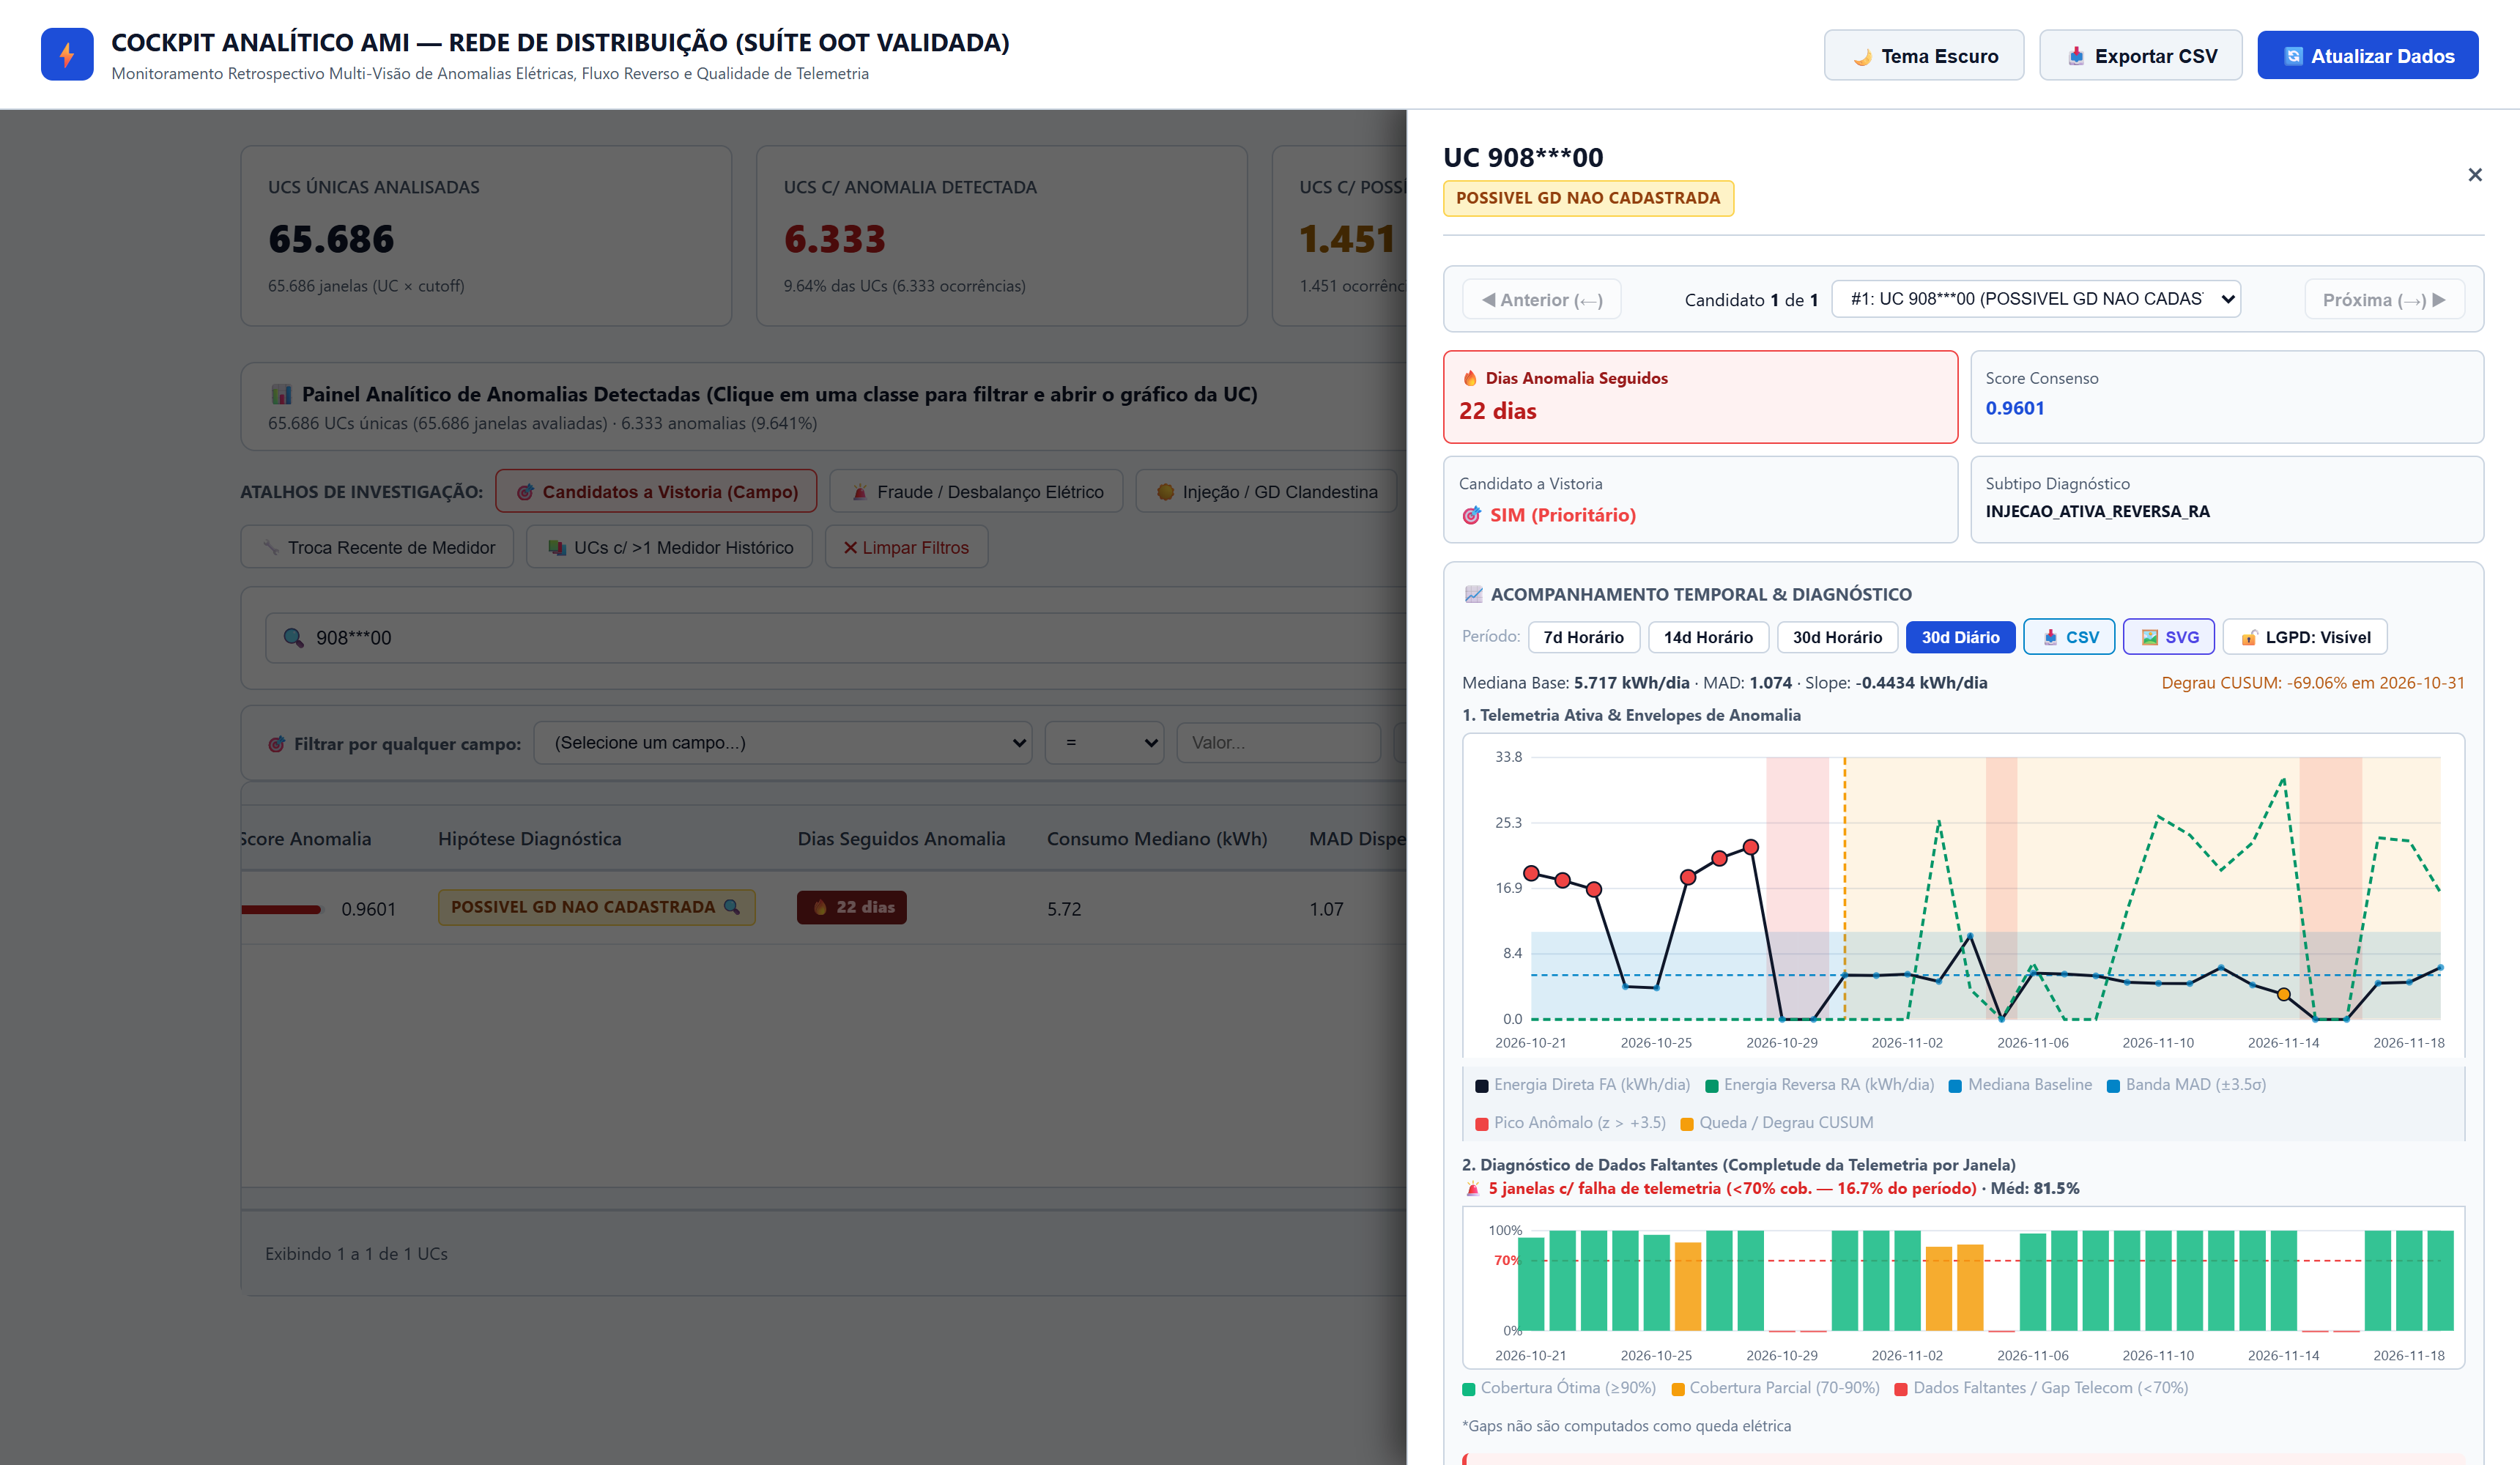
\includegraphics[width=0.98\textwidth]{manuscript_figures/platform_interfaces/fig_4_4d_cockpit_raiox_uc_908xxx00.png}
  \caption{Painel individual (\emph{Raio-X}) do Cockpit Analítico Web para a UC \texttt{908***00} em janela diária de 30 dias até 19/11/2026, integrando séries de energia ativa direta (FA), reversa (RA), degrau CUSUM e diagnóstico de completude.}
  \label{fig:cockpit-raiox-908xxx00}
\end{figure}

As Figuras~\ref{fig:cockpit-carteira-candidatos} e~\ref{fig:cockpit-raiox-908xxx00} ilustram a transição da visão populacional para a análise individual. Na visão de carteira, os indicadores reconciliados distinguem explicitamente candidatos a vistoria (\texttt{6.333}) de unidades retidas em quarentena de comunicação (\texttt{2.829}). Na investigação individual da UC~\texttt{908***00}, o painel exibe simultaneamente o histórico elétrico e a integridade da telemetria, apoiando a etapa de análise humana prévia a eventual decisão de campo.
